%! Author = joels
%! Date = 05/01/2021

\section{MVVM}
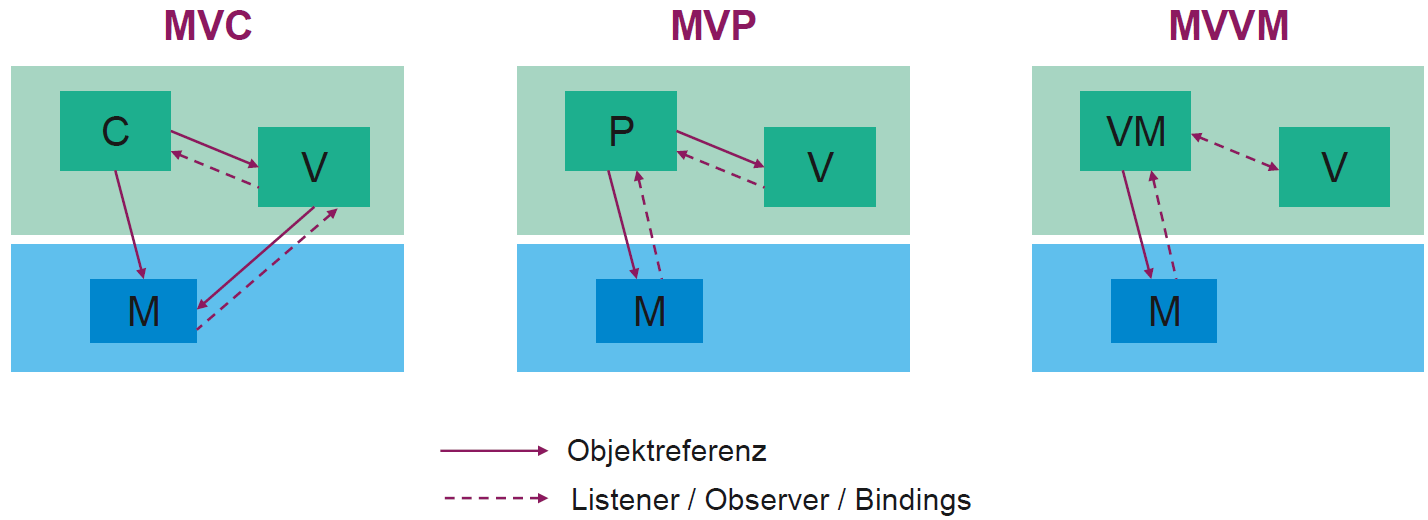
\includegraphics{mvc_mvp_mvvm.png}
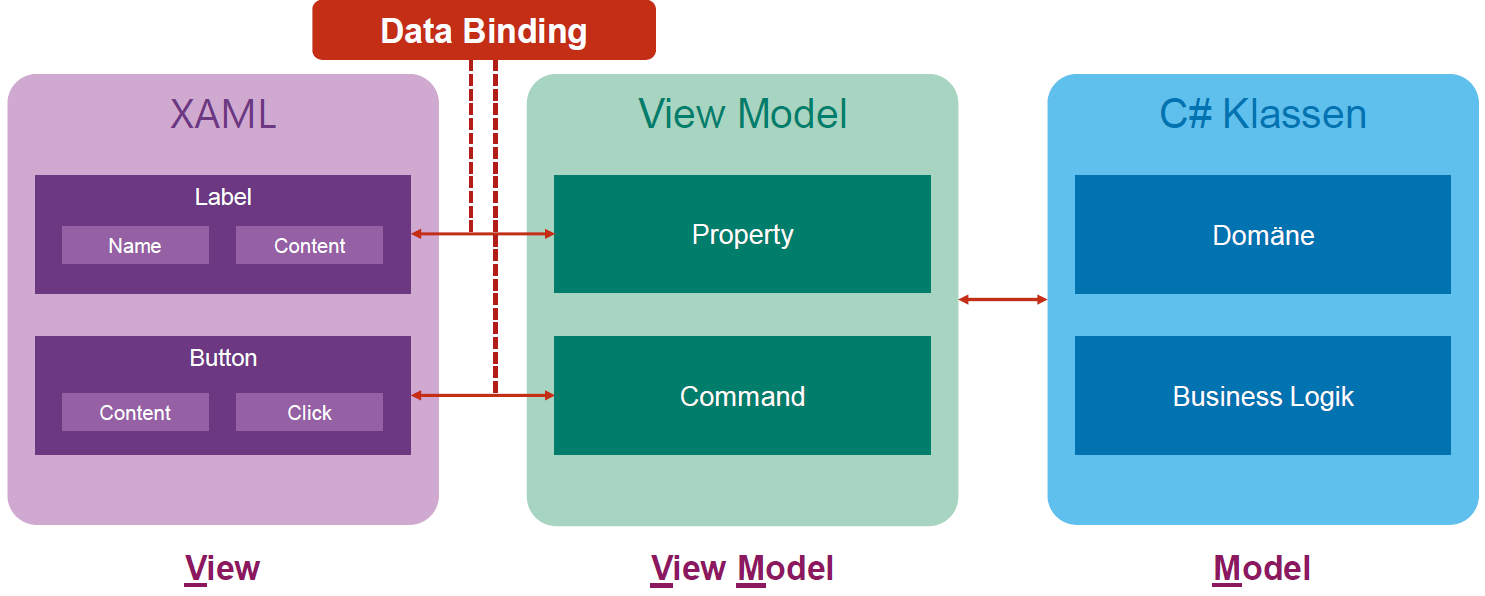
\includegraphics{data_binding_2.png}
\begin{minipage}{0.54\linewidth}
    \textbf{Ziel:}\\
    Trennung von Präsentation und Logik\\
    \textbf{Model:}\\
    Umfasst Domänen-/Businesslogik. C\# Klassen (ggf. mit INPC oder INCC), oft durch Interfaces abstrahiert\\
    \textbf{View:} Kümmert sich um Darstellung. XAML oder Code Behind\\
    \textbf{View Model:} Enthält Darstellungslogik. C\# Klasse mit INPC
\end{minipage}
\begin{minipage}{0.46\linewidth}
    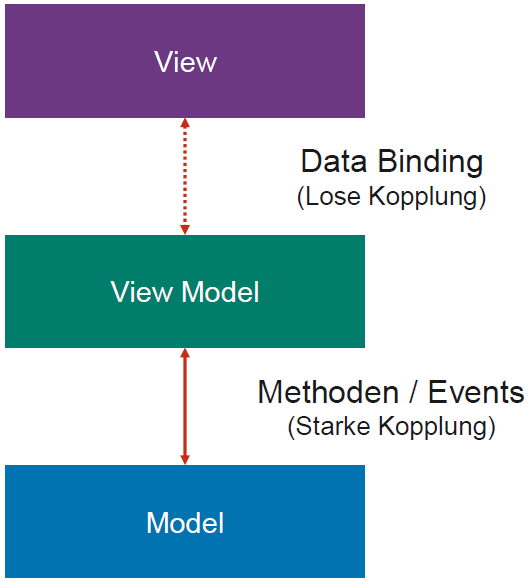
\includegraphics{mvvm_ueberblick.png}
\end{minipage}
\subsection{View Model in WPF}
\textbf{\textcolor{blue}{2 Hauptvarianten: Klassisch (links), Durchgriff (rechts):}}
\begin{center}
    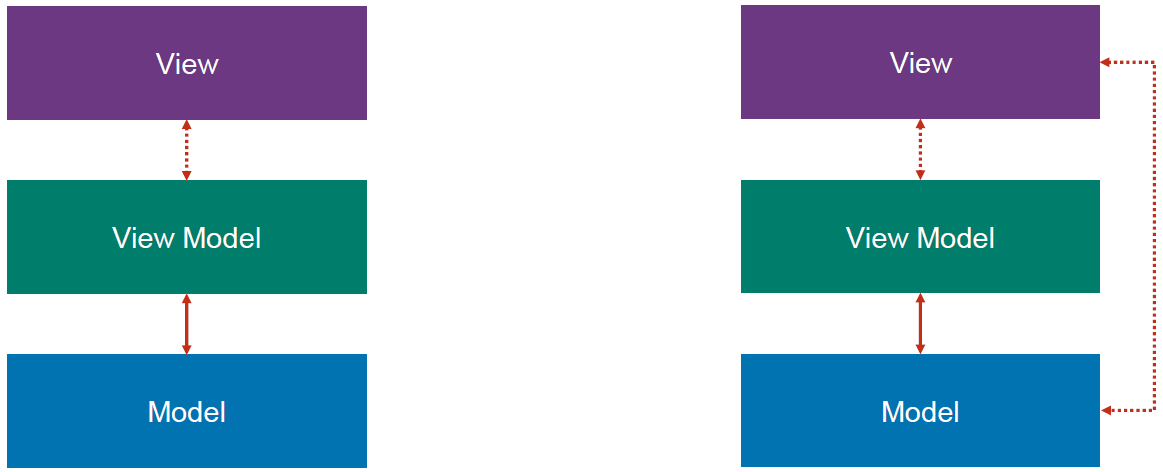
\includegraphics[width=0.75\linewidth]{mvvm_varianten.png}
\end{center}
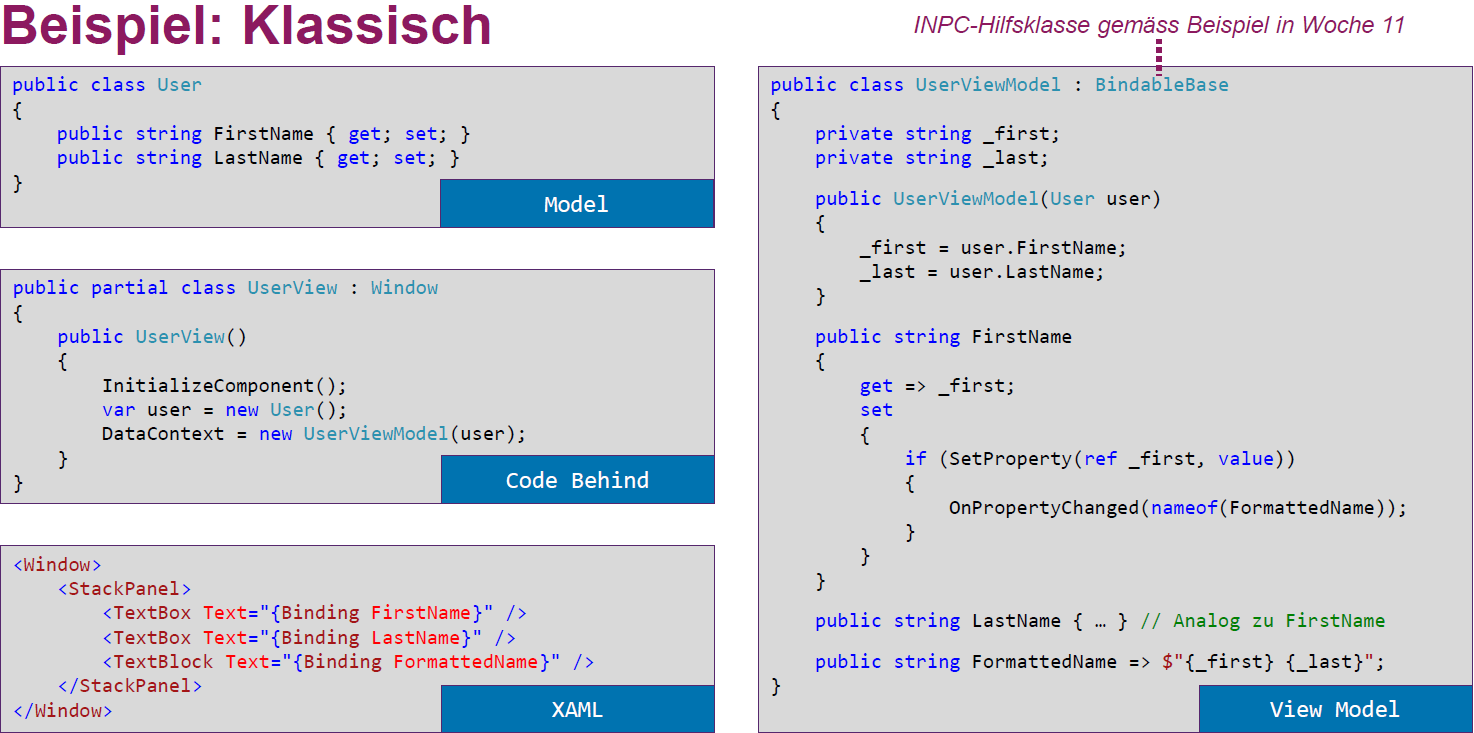
\includegraphics{mvvm_klassisch.png}
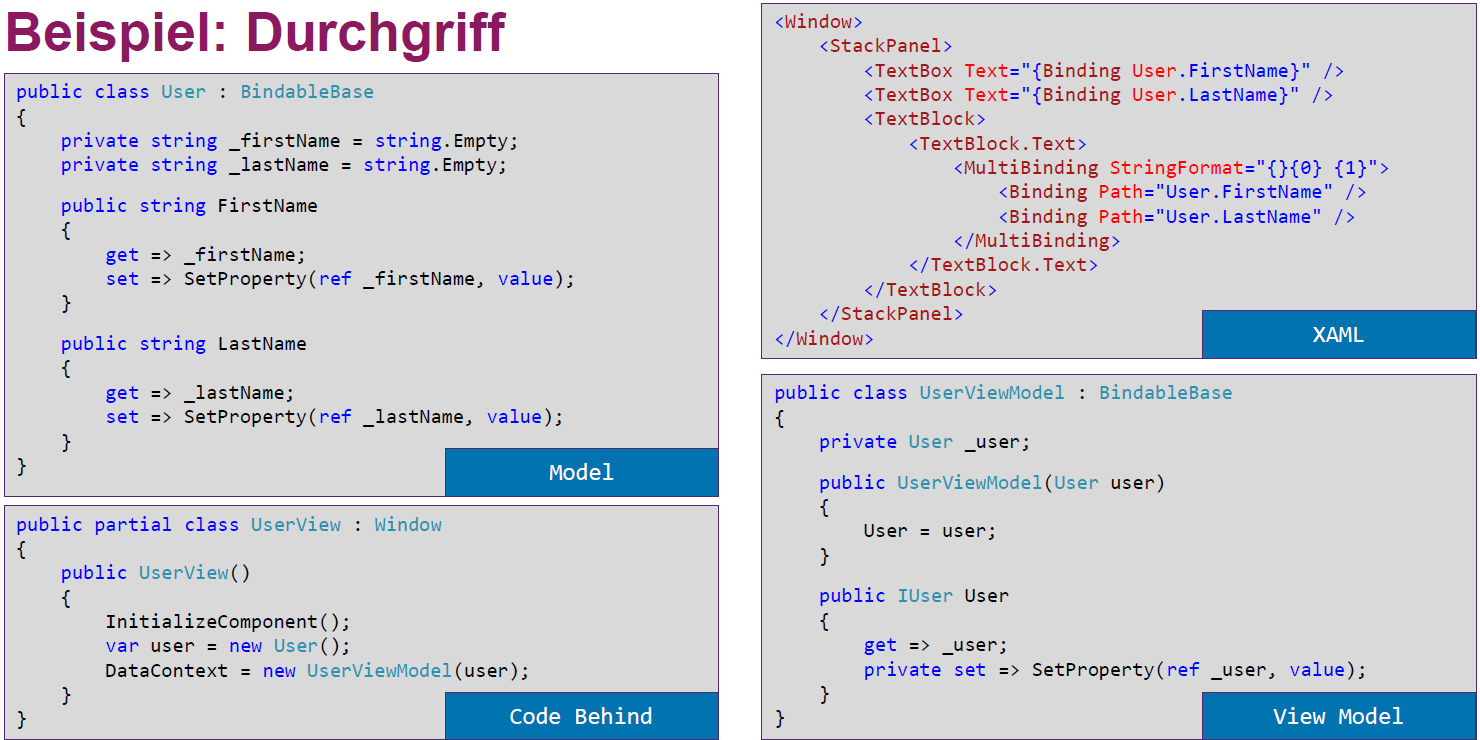
\includegraphics{mvvm_durchgriff.png}
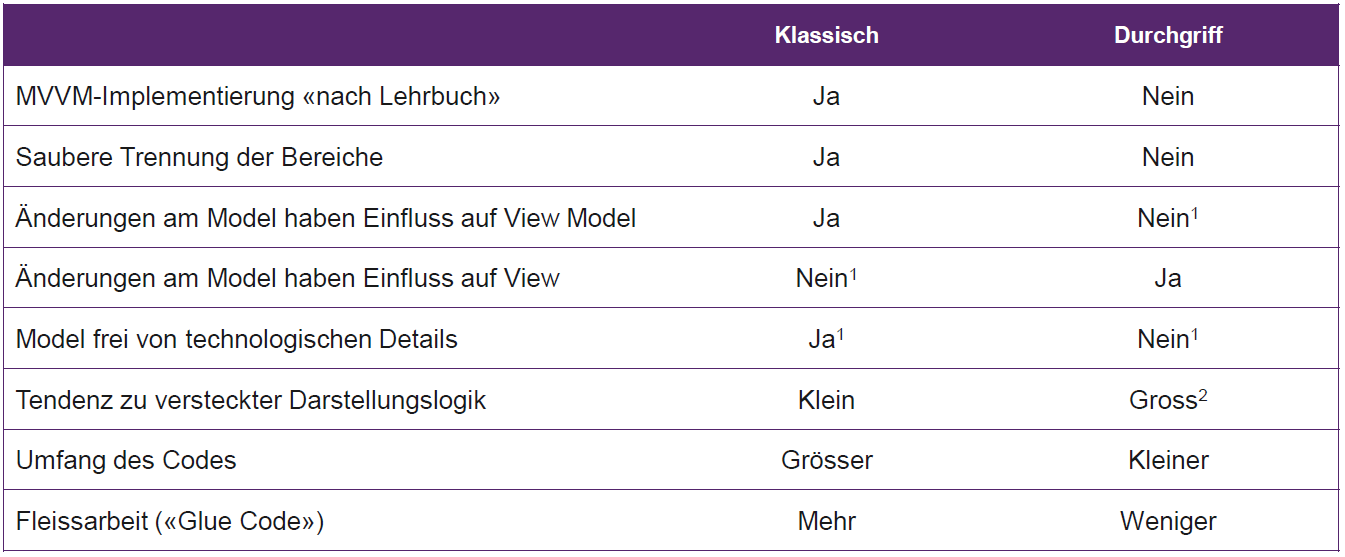
\includegraphics{mvvm_varianten_vergleich.png}
\subsubsection{AutoMapper - Besseres Klassisch}
Hauptnachteil der Variante \dq Klassisch\dq ist der zusätzliche Glue Code. \textcolor{blue}{AutoMapper} ist ein \textcolor{blue}{Objekt-Objekt-Mapper}. Abfüllen des View Models aus dem Model und bei Bedarf zurück. Integration
als NuGet Paket.\\
\textbf{Beispiel:} View Model aus Model erzeugen
\begin{lstlisting}
var config = new MapperConfiguration(cfg => cfg.CreateMap<User, UserViewModel>());
var mapper = config.CreateMapper();
var viewModel = mapper.Map<UserViewModel>(user);
\end{lstlisting}
\subsubsection{Aktionen in View Models}
Data Binding erlaubt die Verknüpfung von Eigenschaften, nicht aber von Methoden. Methoden müssen in Objekte verpackt werden.\\
\textcolor{blue}{ICommand} definiert die Schnittstelle für solche Objekte. View Models stellen ICommand-Objekte zur Verfügung.\\
Command-Eigenschaft von Controls wird an ICommand-Objekte gebunden: Button, Checkbox, RadioButton etc.
\subsubsection{ICommand}
\textbf{\textcolor{blue}{Execute(Object parameter):}} Enthält den Code der auszuführenden Aktion. Bsp: Alter eines Benutzers verringern\\
\textbf{\textcolor{blue}{CanExecute(Object parameter):}} Prüft, ob die Aktion ausgeführt werden kann. Steuert bei einigen Controls die Verfügbarkeit (IsEnabled). Bsp: true, falls Alter grösser als 0, sonst false\\
\textbf{\textcolor{blue}{CanExecuteChanged:}} Auszulösen, wenn Bedingung in CanExecute() sich ändert. Bsp: Nach jeder Änderung des Alters\\
\textbf{\textcolor{blue}{Beispiel ohne Hilfsmittel:}}
\begin{lstlisting}
// Command
public class DecreaseAgeCommand : ICommand {
    private readonly UserViewModel _viewModel;
    public DecreaseAgeCommand(UserViewModel viewModel) {
        _viewModel = viewModel;
    }
    public bool CanExecute(object parameter) {
        return _viewModel.Age > 0;
    }
    public void Execute(object parameter) {
        _viewModel.Age--;
        OnCanExecuteChanged();
    }
    public event EventHandler CanExecuteChanged;
    protected virtual void OnCanExecuteChanged() {
        CanExecuteChanged?.Invoke(this, EventArgs.Empty);
    }
}
// View Model:
// View Model zwecks Lesbarkeit gekürzt
public class UserViewModel : BindableBase {
    public UserViewModel(User user) {
        DecreaseAgeCommand = new DecreaseAgeCommand(this);
    }
    public int Age {
        get => ... ;
        set => ... ;
    }
    public ICommand DecreaseAgeCommand { get; }
}

// XAML
<Window>
    <StackPanel>
        <Button Content="Decrease Age"
            Command="{Binding DecreaseAgeCommand}" />
    </StackPanel>
</Window>
\end{lstlisting}
\textbf{\textcolor{blue}{Beispiel mit Hilfsklasse:}}
\begin{lstlisting}
// Relay Command
public sealed class RelayCommand : ICommand {
  private readonly Action _execute;
  private readonly Func<bool> _canExec;
  public RelayCommand(Action execute, Func<bool>canExec){
    _execute = execute;
    _canExec = canExec;
  }
  public bool CanExecute(object parameter) => _canExec();
  public void Execute(object parameter) => _execute();
  public event EventHandler CanExecuteChanged;
  public void RaiseCanExecuteChanged() {
    CanExecuteChanged?.Invoke(this, EventArgs.Empty);
  }
}

// View Model
public class UserViewModel : BindableBase {
    public UserViewModel(User user) {
        DecreaseAgeCommand = new RelayCommand(OnDecreaseAge, CanDecreaseAge);
    }
    public int Age {
        get => ... ;
        private set => ... ;
    }
    public ICommand DecreaseAgeCommand { get; }
    private bool CanDecreaseAge() => Age > 0;
    private void OnDecreaseAge() {
        Age--;
        DecreaseAgeCommand.RaiseCanExecuteChanged();
    }
}
\end{lstlisting}
\subsubsection{Relay Command}
\textbf{Vorteile des Relay Command:} ICommand Interface einmalig implementiert. Universell verwendbar. Command-Code näher beim View Model.\\
\textbf{Nachteile des Relay Command:} Keine wiederverwendbaren Command-Klassen.
\subsubsection{Commands mit Parametern}
\textbf{Commands können Parameter übernehmen:}\\
\textcolor{blue}{Execute(Object parameter)} und \textcolor{blue}{CanExecute(Object parameter)}. Der Parameter wird in der View gebunden: Attribut \textcolor{blue}{CommandParameter}.
\begin{lstlisting}
<Window>
    <StackPanel>
        <Button Content="Show Details"
            Command="{Binding ShowDetailsCommand}"
            CommandParameter="{Binding SelectedUser}" />
    </StackPanel>
</Window>
\end{lstlisting}

\subsection{Tipps für die Umsetzung}
\subsubsection{Zuteilen der Logik}
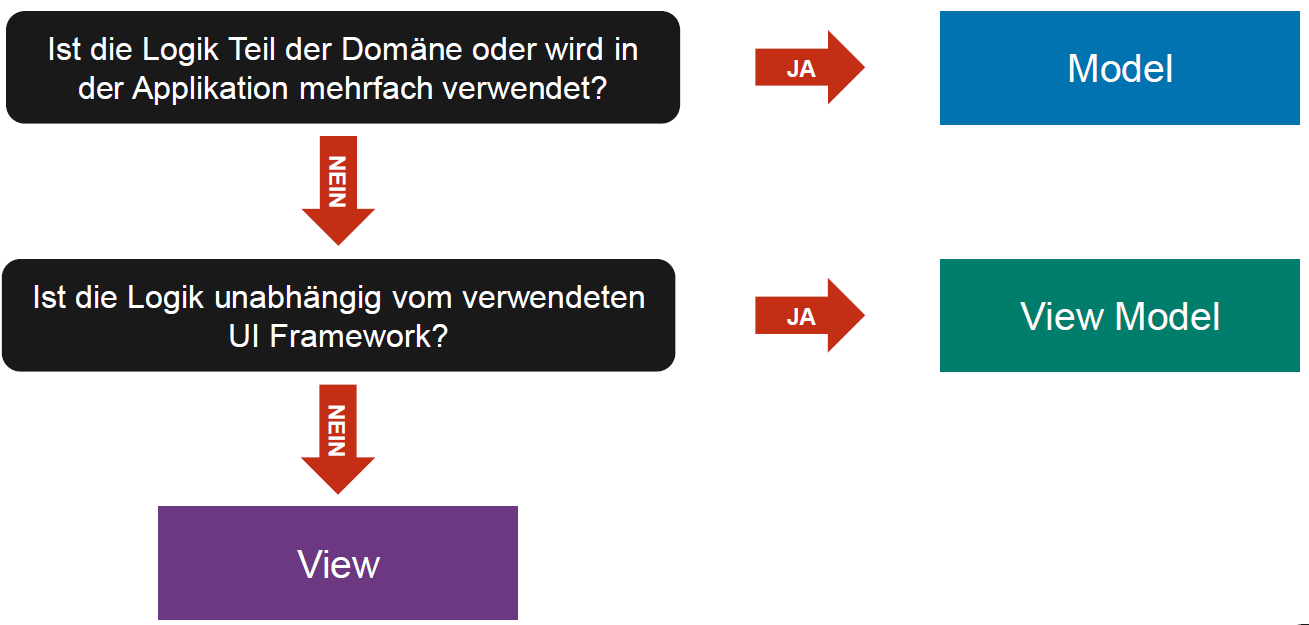
\includegraphics{mvvm_umsetzung.png}
\subsubsection{Erzeugung von Views und View Models}
Das View Model koordiniert den Applikationsfluss.\\
\textbf{Beispiel: Öffnen eines Fensters:}
\begin{itemize}[topsep=0pt, leftmargin=4mm]
    \setlength\itemsep{-0.3em}
    \item 1. Command auf View Model aufrufen (Binding)
    \item 2. Command-Logik löst bei Erfolg ein \dq Navigation Event\dq für die Event aus
    \item 3. Der Event Handler in View A erzeugt View B und zeigt diese an (Window.Show)
    \item 4. View B erzeugt in Konstruktor sein View Model und übernimmt den Applikationsfluss
\end{itemize}
\subsubsection{Hilfsmittel für Model}
\begin{itemize}[topsep=0pt, leftmargin=4mm]
    \setlength\itemsep{-0.3em}
    \item Empfohlene O/R-Mapping-Technologie für .NET Anwendungen
    \item Unterschiedliche Entwicklungsansätze
    \begin{itemize}[topsep=0pt, leftmargin=4mm]
        \setlength\itemsep{-0.3em}
        \item \textbf{Model-First:} Erstellung des Modells in visuellem Editor
        \item \textbf{Database-First:} Erstellung der Datenbank mit SQL
        \item \textbf{Code-First:} Erstellung des Modells mit attributierten POCO's
    \end{itemize}
\end{itemize}